
% !TEX program = xelatex
% ============================================================
%  DeepFool 对抗攻击 —— 详细讲解 Beamer 文稿
%  编译方式：xelatex deepfool.tex （需运行两次以生成目录/参考文献）
%
%  本文件使用 fontspec + Noto CJK 字体，无需 ctex 宏包，通用性强。
%  如果你的环境装了 ctex，也可以把下面前导区换成：
%      \documentclass[aspectratio=169]{ctexbeamer}
%  并删去 fontspec / XeTeXlinebreaklocale 相关四行即可。
% ============================================================
\documentclass[aspectratio=169,11pt]{beamer}

% ---------- 中文支持（fontspec 方案，XeLaTeX 编译） ----------
\usepackage{fontspec}
\setmainfont{Noto Serif CJK SC}
\setsansfont{Noto Sans CJK SC}
\XeTeXlinebreaklocale "zh"
\XeTeXlinebreakskip=0pt plus 1pt minus 0.1pt

% ---------- 数学与图表宏包 ----------
\usepackage{amsmath,amssymb,mathtools}
\usepackage{booktabs}
\usepackage{graphicx}
\usepackage{tikz}
\usetikzlibrary{arrows.meta,calc,positioning}

% ---------- 主题 ----------
\usetheme{Madrid}
\setbeamertemplate{navigation symbols}{}
\setbeamertemplate{caption}[numbered]

% ---------- 数学算子 ----------
\DeclareMathOperator*{\argmin}{arg\,min}
\DeclareMathOperator*{\argmax}{arg\,max}
\DeclareMathOperator{\sign}{sign}
\newcommand{\norm}[1]{\left\lVert #1 \right\rVert}
\newcommand{\bx}{\boldsymbol{x}}
\newcommand{\br}{\boldsymbol{r}}
\newcommand{\bw}{\boldsymbol{w}}

% ---------- 标题信息 ----------
\title[DeepFool 对抗攻击]{DeepFool：一种简洁而精确的对抗攻击方法}
\subtitle{寻找最小扰动的几何视角}
\author{汇报人}
\institute{对抗攻击实验课程}
\date{\today}

% ---------- 每章前插入目录页 ----------
\AtBeginSection[]{
  \begin{frame}{本章内容}
    \tableofcontents[currentsection]
  \end{frame}
}

\begin{document}

% ============ 封面 ============
\begin{frame}
  \titlepage
\end{frame}

% ============ 目录 ============
\begin{frame}{目录}
  \tableofcontents
\end{frame}

% ================================================================
\section{背景与动机}
% ================================================================

\begin{frame}{什么是对抗样本？}
  \begin{block}{核心现象}
    给一张能被模型正确分类的图像，叠加一个\textbf{人眼几乎察觉不到}的微小扰动，
    模型就会以高置信度把它分错。这个被扰动后的图像称为\textbf{对抗样本}。
  \end{block}
  \vspace{0.5em}
  \begin{itemize}
    \item 扰动 $\br$ 很小：$\norm{\br}$ 接近 0，视觉上与原图无差别。
    \item 但模型输出 $\hat k(\bx+\br) \neq \hat k(\bx)$。
    \item 说明深度网络的决策边界在高维空间里非常“贴近”正常样本。
  \end{itemize}
  \vspace{0.5em}
  \alert{研究意义：} 评估模型鲁棒性、理解决策边界、改进训练（对抗训练）。
\end{frame}

\begin{frame}{对抗攻击的形式化定义}
  对于分类器 $f$ 与样本 $\bx$，记其预测标签
  \[
    \hat k(\bx) = \argmax_k f_k(\bx).
  \]
  寻找“最小”对抗扰动可写成优化问题：
  \[
    \Delta(\bx;f) \;:=\; \min_{\br}\; \norm{\br}_2
    \quad \text{s.t.}\quad \hat k(\bx+\br) \neq \hat k(\bx).
  \]
  \begin{itemize}
    \item $\Delta(\bx;f)$ 度量了样本 $\bx$ 到\textbf{决策边界}的距离。
    \item 这个距离越小，说明模型在该点越“脆弱”。
    \item \textbf{DeepFool 的目标：} 高效、准确地求解这个最小扰动。
  \end{itemize}
\end{frame}

\begin{frame}{回顾 FGSM 及其局限}
  最经典的攻击 FGSM（Fast Gradient Sign Method）只走一步：
  \[
    \br = \varepsilon \cdot \sign\!\big(\nabla_{\bx} J(\theta,\bx,y)\big).
  \]
  \begin{itemize}
    \item \textbf{优点：} 单步、极快，直觉清晰（沿损失上升最快方向推一步）。
    \item \textbf{局限一：} 取 $\sign$ 把每个像素都顶到 $\pm\varepsilon$，扰动\textbf{粗糙且偏大}。
    \item \textbf{局限二：} 不是为“最小扰动”设计的，$\varepsilon$ 需要\textbf{手动调}。
  \end{itemize}
  \vspace{0.4em}
  \begin{exampleblock}{由此引出 DeepFool}
    能不能不手调参数，自动找到\textbf{刚好越过决策边界}的最小扰动？
  \end{exampleblock}
\end{frame}

% ================================================================
\section{核心思想（几何直觉）}
% ================================================================

\begin{frame}{几何直觉：决策边界就是“超平面”}
  \begin{itemize}
    \item 在样本附近，把分类器\textbf{局部线性化}，决策边界近似为一个个\textbf{超平面}。
    \item 让样本改变类别，最省力的做法是：沿\textbf{垂直方向}推到\textbf{最近}的那个边界外。
    \item 这正是“点到平面的最短距离”——线性代数里的经典问题。
  \end{itemize}
  \vspace{0.3em}
  \begin{center}
  \begin{tikzpicture}[>=Stealth, scale=0.95]
    % 最近边界（较陡的线，离 x 近）
    \draw[thick,gray] (1.7,-1.6) -- (2.1,1.8);
    % 较远边界（较平的线，离 x 远）
    \draw[thick,gray] (-1.8,2.7) -- (3.8,3.1);
    % 样本点 x
    \fill (0,0) circle (2.5pt);
    \node[below left] at (0,0) {$\bx$};
    % 选中的最小扰动：指向最近边界
    \draw[->,very thick,orange!85!red] (0,0) -- (1.97,0.03)
      node[midway,above] {\small $\br_*$（最小）};
    % 被舍弃的更远方向
    \draw[->,thick,gray,dashed] (0,0) -- (0,2.92)
      node[midway,right] {\small 更远 → 舍弃};
    % 区域标注
    \node at (-1.25,-1.1) {\small class A（当前）};
    \node at (3.0,-0.7) {\small class B};
    \node at (-1.1,3.4) {\small class C};
  \end{tikzpicture}
  \end{center}
  \footnotesize 在所有相邻类别的边界中，DeepFool 选择\textbf{最近}的那条，做垂直投影。
\end{frame}

% ================================================================
\section{数学推导}
% ================================================================

\begin{frame}{二分类：线性分类器（最简单情形）}
  设二分类器 $f(\bx)=\bw^\top\bx + b$，预测 $\hat k(\bx)=\sign\!\big(f(\bx)\big)$。
  \vspace{0.4em}

  样本 $\bx$ 到超平面 $\{\,\bx: f(\bx)=0\,\}$ 的最小扰动，就是\textbf{正交投影}：
  \[
    \boxed{\;\br_*(\bx) = -\,\frac{f(\bx)}{\norm{\bw}_2^{2}}\,\bw\;}
  \]
  \begin{itemize}
    \item 方向：沿法向量 $\bw$（边界的垂直方向）。
    \item 大小：$\norm{\br_*}_2 = \dfrac{|f(\bx)|}{\norm{\bw}_2}$，正是\textbf{点到平面的距离}。
    \item 这是闭式解，一步到位。
  \end{itemize}
\end{frame}

\begin{frame}{二分类：一般（非线性）分类器}
  真实网络是非线性的，没有全局超平面。DeepFool 的做法：\textbf{反复线性化 + 迭代}。
  \vspace{0.4em}

  在当前迭代点 $\bx_i$ 把 $f$ 一阶展开：
  \[
    f(\bx_i + \br) \approx f(\bx_i) + \nabla f(\bx_i)^\top \br .
  \]
  令其等于 0，得到这一步的最小扰动：
  \[
    \br_i = -\,\frac{f(\bx_i)}{\norm{\nabla f(\bx_i)}_2^{2}}\,\nabla f(\bx_i),
    \qquad \bx_{i+1} = \bx_i + \br_i .
  \]
  \begin{itemize}
    \item 每走一步都重新计算梯度（重新线性化），逼近真实弯曲的边界。
    \item 直到 $\hat k(\bx_i)$ 改变为止，通常只需 \textbf{2--4 步}。
  \end{itemize}
\end{frame}

\begin{frame}{多分类：在所有边界中选最近的一条}
  对 $c$ 类分类器 $f:\mathbb{R}^n\to\mathbb{R}^c$，记原始标签 $\hat k(\bx_0)$。
  在迭代点 $\bx_i$，对每个其他类别 $k \neq \hat k(\bx_0)$ 定义：
  \[
    \bw'_k = \nabla f_k(\bx_i) - \nabla f_{\hat k(\bx_0)}(\bx_i),
    \qquad
    f'_k = f_k(\bx_i) - f_{\hat k(\bx_0)}(\bx_i).
  \]
  \begin{itemize}
    \item $\bw'_k$：类别 $k$ 与当前类之间“等分边界”的法向。
    \item $f'_k$：当前点相对该边界的“带符号距离量”。
  \end{itemize}
  \vspace{0.3em}
  选出\textbf{最近}的边界：
  \[
    \hat l = \argmin_{k \neq \hat k(\bx_0)} \frac{|f'_k|}{\norm{\bw'_k}_2}.
  \]
\end{frame}

\begin{frame}{多分类：最小扰动公式}
  朝最近边界 $\hat l$ 做正交投影，得到本步扰动：
  \[
    \boxed{\;
      \br_i = \frac{|f'_{\hat l}|}{\norm{\bw'_{\hat l}}_2^{2}}\,\bw'_{\hat l}
    \;}
  \]
  然后更新 $\bx_{i+1} = \bx_i + \br_i$，重复直到类别改变。
  \vspace{0.6em}

  最终累计扰动并做\textbf{过冲}（overshoot），确保确实越过边界：
  \[
    \hat\br = (1+\eta)\sum_i \br_i,
    \qquad \eta = 0.02 .
  \]
  \footnotesize 过冲系数 $1.02$ 让扰动“多推一点点”，避免样本卡在边界上、因数值/量化又被推回正确类。
\end{frame}

% ================================================================
\section{算法与实现}
% ================================================================

\begin{frame}{算法伪代码（多分类 DeepFool）}
  \begin{block}{}
  \footnotesize
  \begin{enumerate}
    \item 初始化 $\bx_0 \gets \bx$，$\ i \gets 0$
    \item \textbf{while} $\hat k(\bx_i) = \hat k(\bx_0)$ \textbf{do}
    \item \quad \textbf{for} $k \neq \hat k(\bx_0)$:
          \ $\bw'_k \gets \nabla f_k(\bx_i) - \nabla f_{\hat k(\bx_0)}(\bx_i)$,
          \ $f'_k \gets f_k(\bx_i) - f_{\hat k(\bx_0)}(\bx_i)$
    \item \quad 选最近边界 \ $\hat l \gets \argmin\limits_{k \neq \hat k(\bx_0)} \dfrac{|f'_k|}{\norm{\bw'_k}_2}$
    \item \quad $\br_i \gets \dfrac{|f'_{\hat l}|}{\norm{\bw'_{\hat l}}_2^{2}}\,\bw'_{\hat l}$,
          \ \ $\bx_{i+1} \gets \bx_i + \br_i$,
          \ \ $i \gets i+1$
    \item \textbf{end while}
    \item \textbf{return} \ $\hat\br = (1+\eta)\sum_i \br_i$
  \end{enumerate}
  \end{block}
  \footnotesize 复杂度主要来自每步对 $c$ 个类别求梯度；CIFAR-10（$c=10$）规模下很快。
\end{frame}

\begin{frame}{实现细节与注意事项}
  \begin{itemize}
    \item \textbf{过冲系数} $\eta=0.02$：保证越界，缓解“边界样本被量化推回”的问题。
    \item \textbf{终止条件}：标签改变即停；另设最大迭代次数（如 50）防止极少数不收敛。
    \item \textbf{范数选择}：默认 $L_2$；可推广到 $L_\infty$ 等 $L_p$ 范数（改投影方式）。
    \item \textbf{无定向攻击}：只保证“分错成某个其他类”，不能指定目标类。
    \item \textbf{数值实现}：把图像当作向量，逐步累加 $\br_i$，最后裁剪到合法像素区间 $[0,1]$。
  \end{itemize}
  \vspace{0.3em}
  \begin{exampleblock}{常用工具}
    可直接用 \texttt{torchattacks}、\texttt{Foolbox}、\texttt{ART} 等库调用 DeepFool，几行即可跑通。
  \end{exampleblock}
\end{frame}

% ================================================================
\section{实验效果与对比}
% ================================================================

\begin{frame}{鲁棒性度量指标 $\hat\rho_{adv}$}
  论文用\textbf{平均相对扰动}衡量模型的鲁棒性：
  \[
    \hat\rho_{adv}(f) = \frac{1}{|\mathcal{D}|}
      \sum_{\bx \in \mathcal{D}} \frac{\norm{\hat\br(\bx)}_2}{\norm{\bx}_2}.
  \]
  \begin{itemize}
    \item 分子：DeepFool 找到的最小扰动范数；分母：原图范数（归一化）。
    \item $\hat\rho_{adv}$ \textbf{越小}，说明只需更小扰动即可骗过模型 $\Rightarrow$ 模型越脆弱。
    \item 它给出了一个\textbf{与攻击者超参无关}的、可比较的鲁棒性数值。
  \end{itemize}
\end{frame}

\begin{frame}{与 FGSM 的对比}
  \begin{table}
  \centering
  \begin{tabular}{lcccc}
    \toprule
    方法 & 步数 & 扰动范数 & 骗过率 & 是否需调参 \\
    \midrule
    FGSM     & 单步       & 大           & 高   & 需手调 $\varepsilon$ \\
    DeepFool & 迭代（2--4） & \alert{小（约 FGSM 的 $1/5$）} & 相当 & 无需 \\
    \bottomrule
  \end{tabular}
  \end{table}
  \vspace{0.6em}
  \begin{block}{关键结论}
    论文报告：DeepFool 扰动范数约为 FGSM 的 \textbf{1/5}（ImageNet 上约 1/10），骗过率相当。
    \\[0.3em]
    \alert{本项目实测（下一节）：} 在 ResNet-18/CIFAR-10 上，DeepFool 平均 $L_2$
    仅为 FGSM 的约 \textbf{1/11}（$0.16$ vs $1.72$），骗过率几乎一致。
  \end{block}
\end{frame}

\begin{frame}{本项目实验设置}
  \begin{itemize}
    \item \textbf{模型：} ResNet-18，在 CIFAR-10（$32\times32$ 原生分辨率）上微调。
          干净测试准确率 \textbf{88.53\%}（Top-3 98.14\%）。
    \item \textbf{攻击实现：} \texttt{torchattacks}，全部在 $[0,1]$ 像素空间进行，
          归一化包进模型（避免 clamp 破坏对抗样本）。
    \item \textbf{DeepFool 配置：} \texttt{steps=20}, \texttt{overshoot=0.02}，
          取 200 个测试样本评估。
    \item \textbf{对照攻击：} FGSM、APGD（均 $L_\infty$，$\varepsilon=8/255$），
          统一画扰动分布 / 混淆矩阵 / t-SNE。
    \item \textbf{口径：} 报告\textbf{条件攻击成功率}（只统计干净分对、被攻击翻掉的样本），
          并配对给出 Clean / Robust Acc。
  \end{itemize}
\end{frame}

\begin{frame}{实测结果：三种攻击对比（普通模型，白盒）}
  \begin{table}
  \centering
  \footnotesize
  \begin{tabular}{lcccc}
    \toprule
    攻击 & 范数 / 预算 & 攻击成功率 & Robust Acc & 平均 $L_2$ \\
    \midrule
    FGSM     & $L_\infty,\ 8/255$ & 97.91\% & 1.88\% & 1.7208 \\
    \alert{DeepFool} & \alert{$L_2$（最小扰动）} & \alert{97.21\%} & \alert{2.50\%} & \alert{\textbf{0.1604}} \\
    APGD     & $L_\infty,\ 8/255$ & 100.00\% & 0.00\% & 1.3048 \\
    \bottomrule
  \end{tabular}
  \end{table}
  \vspace{0.5em}
  \begin{itemize}
    \item DeepFool 的平均 $L_2$ 仅 \textbf{0.16}，约为 FGSM（1.72）的 \alert{$1/11$}、APGD（1.30）的 $1/8$。
    \item 三者骗过率都很高，但 DeepFool 用\textbf{小一个量级}的扰动达成同样效果。
    \item 干净准确率均为 89.69\%（200 样本子集口径）。
  \end{itemize}
\end{frame}

\begin{frame}{实测结果：扰动大小分布（FGSM vs DeepFool）}
  \begin{center}
    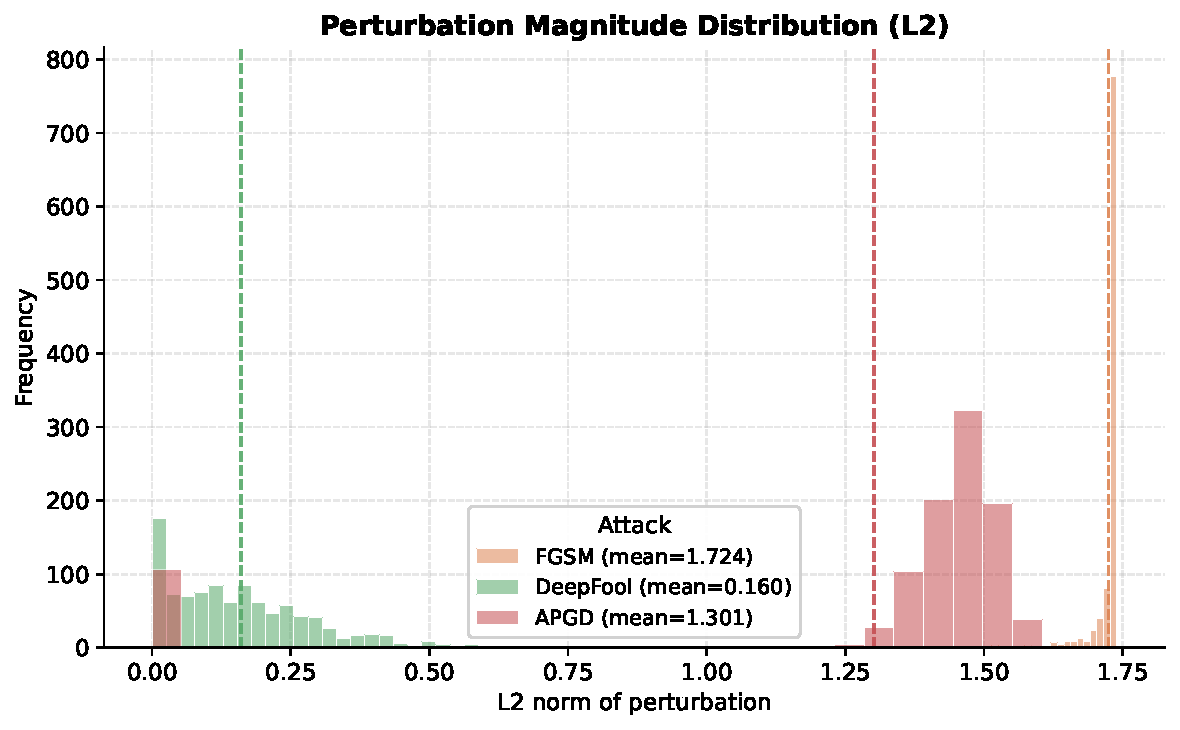
\includegraphics[height=0.66\textheight]{l2_distribution.pdf}
  \end{center}
  \footnotesize
  DeepFool 的 $L_2$ 扰动集中在接近 0 的位置，整体分布远在 FGSM 左侧——
  这正是“最小扰动”路线的直接证据。
\end{frame}

\begin{frame}{实测结果：混淆矩阵（对抗样本上）}
  \begin{columns}[T]
    \begin{column}{0.5\textwidth}
      \centering FGSM\\[0.3em]
      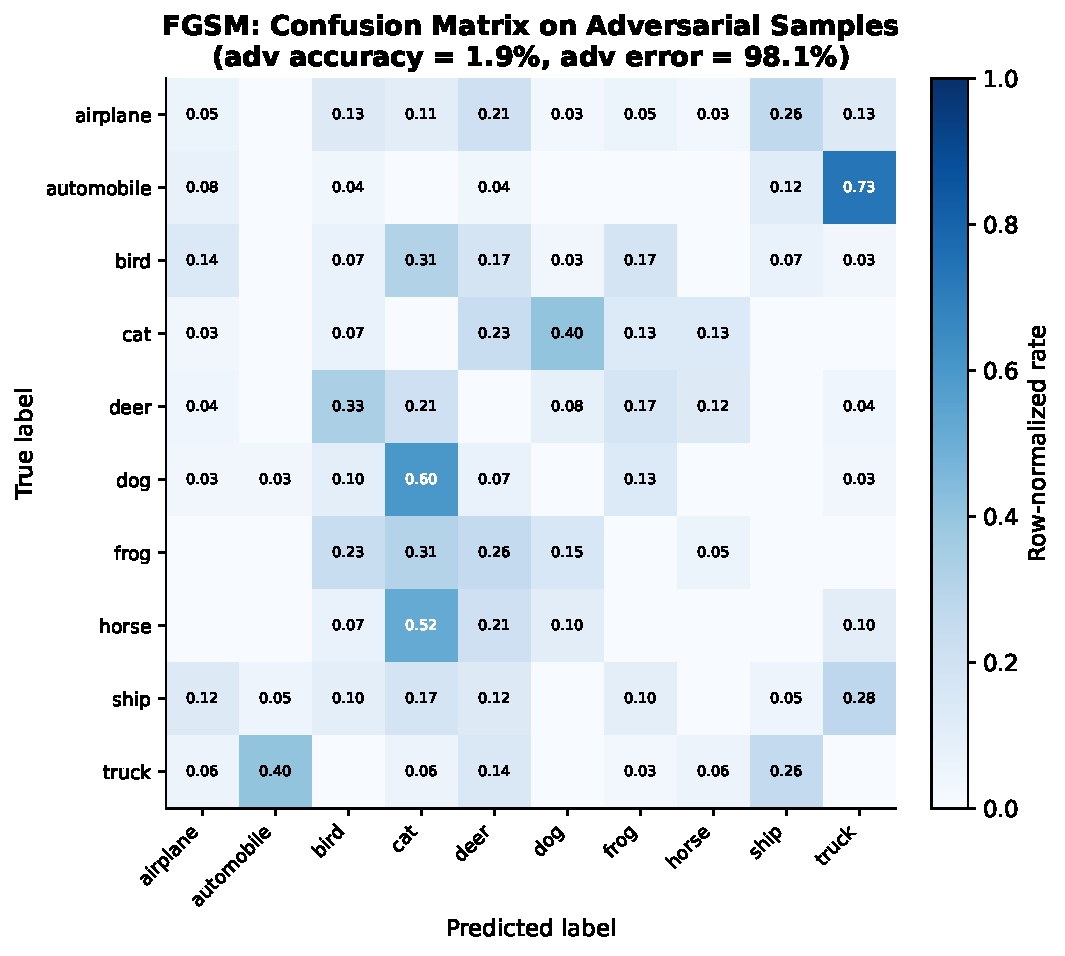
\includegraphics[width=\linewidth]{confusion_fgsm.pdf}
    \end{column}
    \begin{column}{0.5\textwidth}
      \centering DeepFool\\[0.3em]
      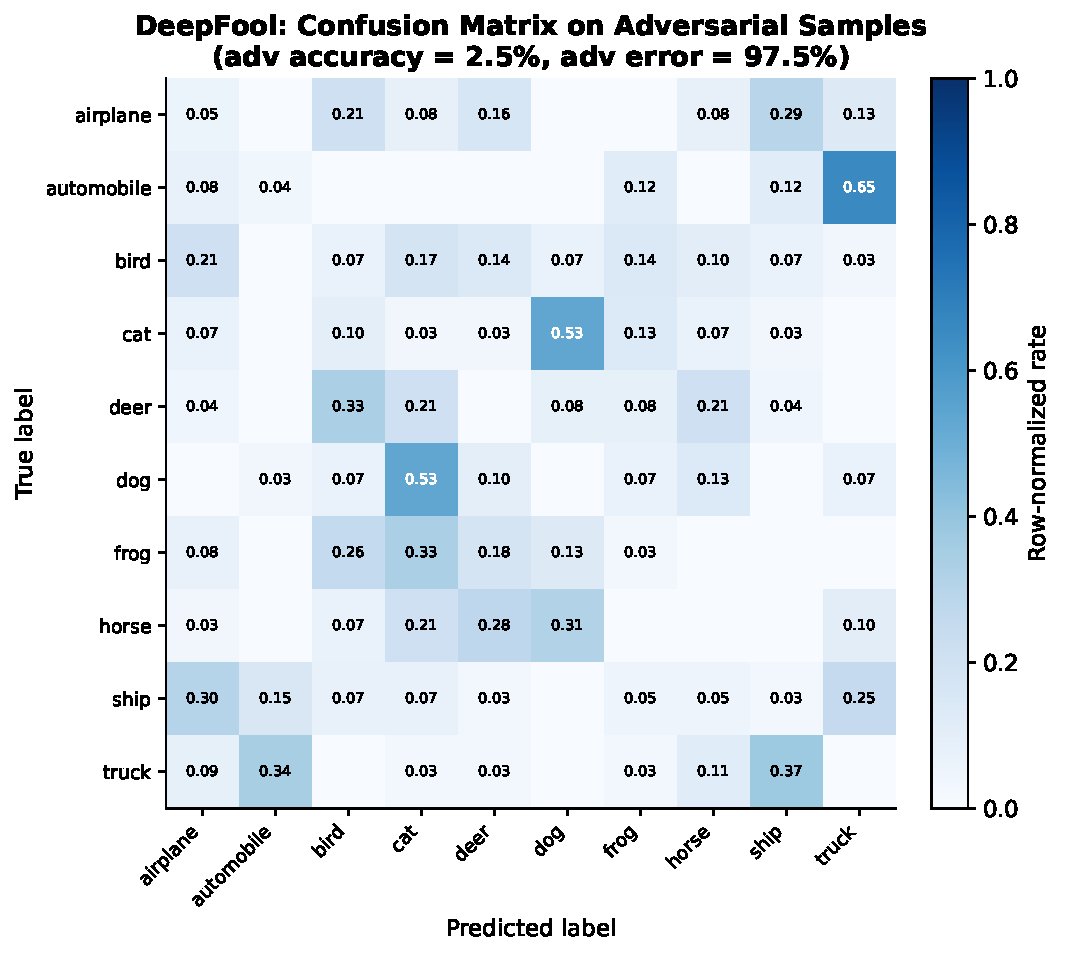
\includegraphics[width=\linewidth]{confusion_deepfool.pdf}
    \end{column}
  \end{columns}
  \vspace{0.3em}
  \footnotesize 对角线（仍分类正确）几乎清空：两种攻击都把样本大量推向\textbf{相邻类别}，
  但 DeepFool 用的扰动小得多。
\end{frame}

\begin{frame}{实测结果：特征空间 t-SNE（Clean vs 对抗）}
  \begin{center}
    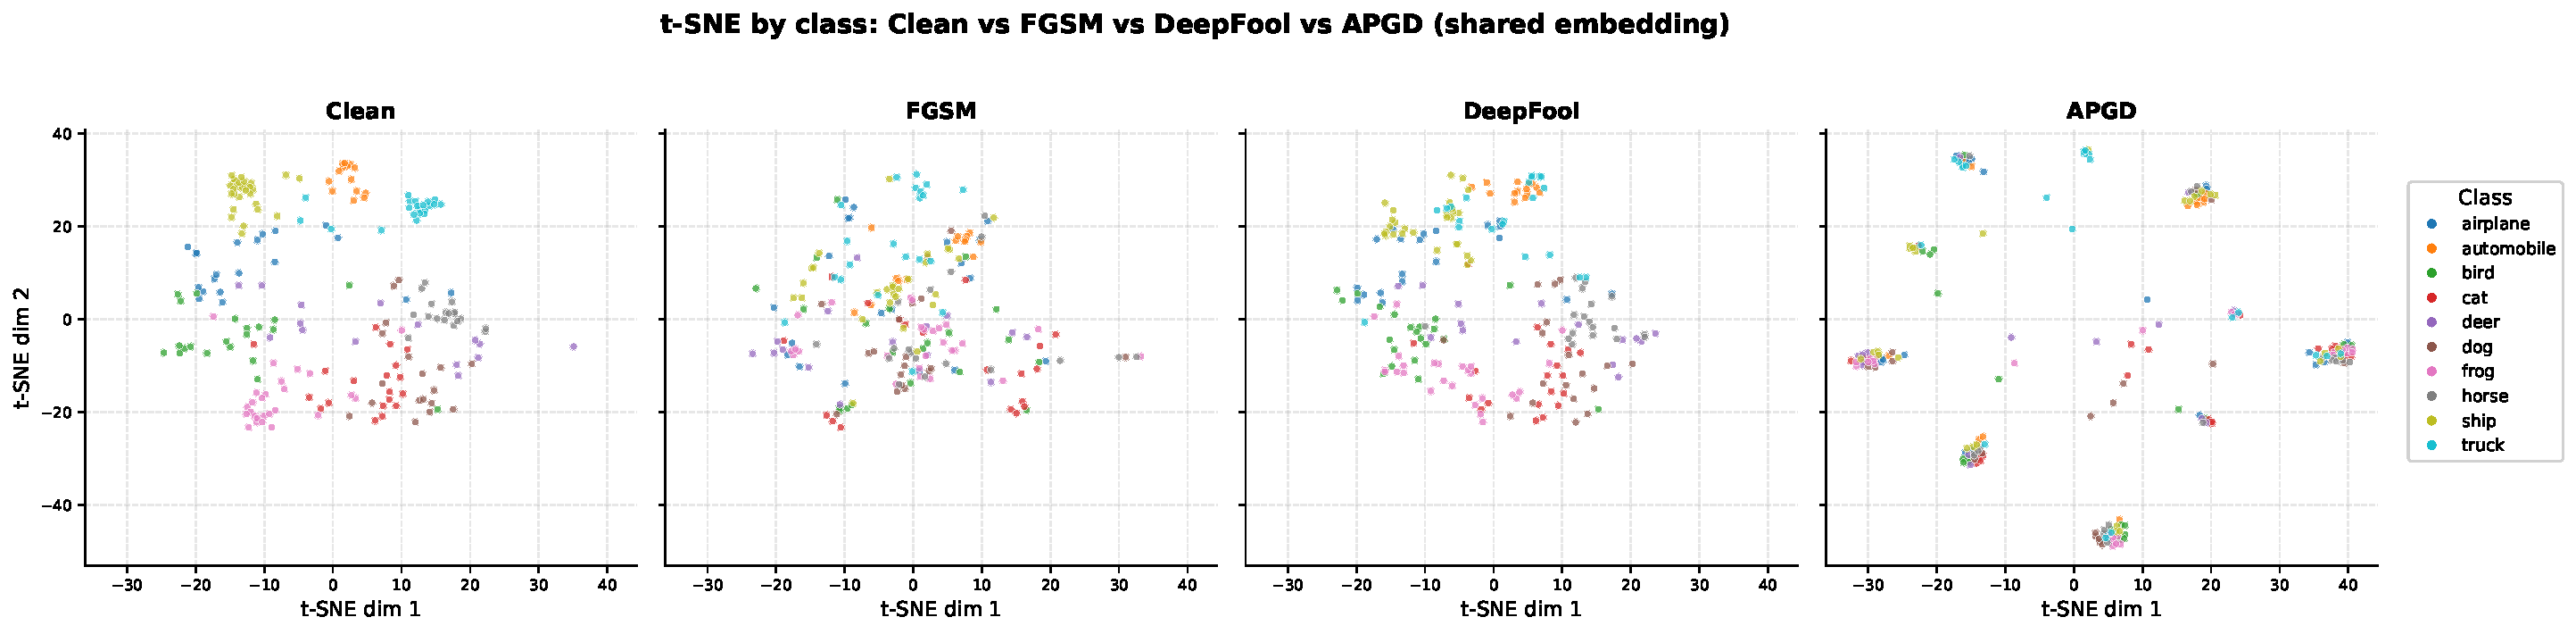
\includegraphics[height=0.66\textheight]{tsne_clean_vs_adv.pdf}
  \end{center}
  \footnotesize
  共享嵌入下，干净样本按类别聚成清晰簇；对抗样本（FGSM/DeepFool/APGD）则被打散、
  跨越到其他类别的区域，直观展示决策被改写。
\end{frame}

% ================================================================
\section{讨论与总结}
% ================================================================

\begin{frame}{优点与局限}
  \begin{columns}[T]
    \begin{column}{0.5\textwidth}
      \begin{block}{优点}
        \begin{itemize}
          \item 扰动\textbf{最小}、几乎不可见
          \item \textbf{无需手调}超参数
          \item 迭代少、\textbf{速度快}
          \item 几何直觉清晰、\textbf{易讲解}
          \item 提供可比的鲁棒性度量
        \end{itemize}
      \end{block}
    \end{column}
    \begin{column}{0.5\textwidth}
      \begin{block}{局限}
        \begin{itemize}
          \item 默认\textbf{无定向}（不能指定目标类）
          \item 扰动卡在边界，\textbf{较“脆”}（易被量化/压缩抵消，靠过冲缓解）
          \item 纯攻击\textbf{强度}略逊于 C\&W
          \item 不专门对抗\textbf{有防御}的模型
        \end{itemize}
      \end{block}
    \end{column}
  \end{columns}
\end{frame}

\begin{frame}{与其他攻击方法的关系}
  \begin{table}
  \centering
  \footnotesize
  \begin{tabular}{lll}
    \toprule
    方法 & 思路 & 特点 \\
    \midrule
    FGSM     & 沿梯度符号走一步     & 单步、$L_\infty$、扰动大 \\
    PGD      & 在 $\varepsilon$ 球内迭代最大化损失 & 迭代、$L_\infty$、很强 \\
    \alert{DeepFool} & \alert{投影到最近决策边界} & \alert{迭代、最小扰动、快、几何} \\
    C\&W     & 优化最小 $L_2$ 扰动   & 最强、扰动极小、较慢 \\
    \bottomrule
  \end{tabular}
  \end{table}
  \vspace{0.6em}
  \begin{itemize}
    \item DeepFool 与 C\&W 同属“\textbf{最小扰动}”路线，但 DeepFool 更快、更直观。
    \item FGSM / PGD 属“\textbf{固定预算}”路线，关注在给定 $\varepsilon$ 内的破坏力。
  \end{itemize}
\end{frame}

\begin{frame}{应用}
  \begin{itemize}
    \item \textbf{鲁棒性评估：} 用平均/中位 $L_2$（或 $\hat\rho_{adv}$）比较不同模型到决策边界的距离——这是 DeepFool 的主要用途。
    \item \textbf{决策边界分析：} 扰动方向揭示了样本最易被推向哪个相邻类别（见混淆矩阵）。
    \item \textbf{不适合用于对抗训练：} DeepFool 求\textbf{最小扰动、刚越界就停}，样本“贴在边界上”、很弱，
          且每个样本扰动大小不一、\textbf{没有统一预算}。
  \end{itemize}
  \vspace{0.3em}
  \begin{exampleblock}{本项目的做法}
    \footnotesize
    训练用 \textbf{PGD-AT}（固定 $\varepsilon$ 内最大化损失，给“最坏情况”样本），
    DeepFool 只作\textbf{评估}。实测对抗训练后，鲁棒模型在 APGD 下 Robust Acc 从
    $0\%$ 升到 $17\%$（代价是干净准确率降到 $72.8\%$）。
  \end{exampleblock}
\end{frame}

\begin{frame}{总结}
  \begin{block}{一句话}
    DeepFool = “反复把样本沿垂直方向，推到\textbf{最近}的决策边界外，所需的\textbf{最小}扰动”。
  \end{block}
  \vspace{0.5em}
  \begin{enumerate}
    \item \textbf{动机：} FGSM 扰动粗糙、需调参 $\Rightarrow$ 求最小扰动。
    \item \textbf{核心：} 局部线性化，边界视为超平面，做正交投影。
    \item \textbf{推导：} 二分类闭式解 $\to$ 迭代 $\to$ 多分类选最近边界。
    \item \textbf{效果：} 扰动约为 FGSM 的 $1/5$，骗过率相当，迭代少、速度快。
  \end{enumerate}
\end{frame}

\begin{frame}{参考文献}
  \footnotesize
  \begin{thebibliography}{9}
    \bibitem{deepfool} S.-M.~Moosavi-Dezfooli, A.~Fawzi, P.~Frossard.
      \emph{DeepFool: a simple and accurate method to fool deep neural networks.} CVPR 2016.
    \bibitem{fgsm} I.~Goodfellow, J.~Shlens, C.~Szegedy.
      \emph{Explaining and Harnessing Adversarial Examples.} ICLR 2015.
    \bibitem{pgd} A.~Madry, A.~Makelov, L.~Schmidt, D.~Tsipras, A.~Vladu.
      \emph{Towards Deep Learning Models Resistant to Adversarial Attacks.} ICLR 2018.
    \bibitem{cw} N.~Carlini, D.~Wagner.
      \emph{Towards Evaluating the Robustness of Neural Networks.} IEEE S\&P 2017.
  \end{thebibliography}
\end{frame}

\begin{frame}[plain]
  \begin{center}
    {\Huge 谢谢！}\\[1em]
    {\large 欢迎提问与讨论}
  \end{center}
\end{frame}

\end{document}
